\section{Overfitting and underfitting}
\label{sec:reg:fit}
\subsection{A small training error is not the destination}
Suppose a sensor measures a periodic signal. In the lecture example [T], the data-generating mechanism is
\begin{equation}
Y=\sin(2\pi X)+\varepsilon,\qquad \E[\varepsilon\mid X]=0,\qquad \Var(\varepsilon\mid X)=\sigma^2.
\label{eq:reg:sine}
\end{equation}
Gaussian noise $\varepsilon\sim\Normal(0,\sigma^2)$ independent of $X$ is one mechanism with these properties. For our constructed experiments, $X$ ranges over $[0,1]$. The underlying mean signal is reproducible; the noise in one measured label is not. A model that memorizes every label may reproduce measurement accidents instead of the signal.

Two different questions are therefore involved: ``How accurately can I reproduce these observations?'' and ``How accurately can I predict a fresh observation?'' The second is the prediction problem. We use the first because the training observations are available, but must check whether that proxy is reliable.

\subsection{Polynomial regression is nonlinear in the input, linear in its coefficients}
The lecture's degree-$M$ family [S1] is
\begin{equation}
f(x,\theta)=\sum_{j=0}^M\theta_jx^j
=\phi_M(x)^\top\theta,\quad
\phi_M(x)=(1,x,\ldots,x^M)^\top\in\R^{M+1}.
\end{equation}
Here $x\in\R$, $\theta\in\R^{M+1}$, and $M\in\{0,1,\ldots\}$. For $M\geq2$ the family permits nonlinear dependence on $x$, but prediction is linear in $\theta$. The degree $M$ is a \emph{hyperparameter} chosen outside coefficient fitting; the $M+1$ coefficients are \emph{parameters} learned from data. A particular fitted degree-$M$ model can have vanishing leading coefficients and hence lower effective polynomial degree.

For observed $\mathcal D=\{(x_i,y_i)\}_{i=1}^N$, put $\Phi_{ij}=x_i^j$ with $j=0,\ldots,M$. Then $\Phi\in\R^{N\times(M+1)}$, $\mathbf y\in\R^N$, and
\begin{equation}
\hat\theta(\mathcal D)\in\argmin_\theta
\hat R_{\mathcal D}(\theta),\qquad
\hat R_{\mathcal D}(\theta)=\frac1N\|\Phi\theta-\mathbf y\|_2^2.
\end{equation}
The slide's sum and this mean have the same minimizers because $N>0$ is fixed. The normalization does matter when reporting errors or later comparing differently scaled penalty terms.
Expanding the squared norm gives
\[
\hat R=\frac1N(\theta^\top\Phi^\top\Phi\theta-2\theta^\top\Phi^\top\mathbf y+\mathbf y^\top\mathbf y),\quad
\nabla_\theta\hat R=\frac2N\Phi^\top(\Phi\theta-\mathbf y).
\]
Thus any minimizer satisfies $\Phi^\top\Phi\hat\theta=\Phi^\top\mathbf y$. Full column rank makes the solution unique. In computation, use a least-squares solver based on QR or SVD instead of explicitly forming an inverse; powers of nearby inputs can produce poorly conditioned columns. With rank deficiency, specify a rule such as the minimum-norm least-squares solution: otherwise ``the learning procedure'' is not fully defined.

\paragraph{Worked example: exact fitting can add unnecessary curvature.}
Take $x=(-1,0,1)$ and measured $y=(1,0,2)$. These are constructed arithmetic data, separate from the sine experiment. The best constant is the mean $1$, giving predictions $(1,1,1)$ and MSE $2/3$. For an affine fit, $\sum_i x_i=0$, so the intercept is $1$ and the slope is
\[
\hat\theta_1=\frac{\sum_i x_i y_i}{\sum_i x_i^2}=\frac{-1+2}{2}=\frac12.
\]
Predictions $(1/2,1,3/2)$ give MSE $(1/4+1+1/4)/3=1/2$. The quadratic $\tfrac12x+\tfrac32x^2$ interpolates all three observations and has training MSE zero. Yet these three training errors alone cannot establish which model predicts future labels best. If the middle label was an unlucky noisy measurement, interpolation preserves that accident.

\paragraph{Try before continuing (A1).} Change only the middle label from $0$ to $1$. Complete the calculation of the new constant and affine fits, then find the interpolating quadratic. Which predictions at $x=0$ move the most? Interpret this as sensitivity to one observation, not yet as a full variance estimate.

\subsection{What model complexity changes}
The degree-$M$ polynomial family is nested inside the degree-$(M+1)$ family: set the extra coefficient to zero. Consequently, on the \emph{same dataset}, the globally minimized unpenalized training error cannot increase with degree. This is a statement about optimal values, not about arbitrary optimizer iterates or a numerically unstable implementation. For $N$ distinct inputs, degree at most $N-1$ can interpolate arbitrary scalar labels. That is enough flexibility to fit noise as well as signal.

A constant cannot follow a full sine wave. A moderate degree can capture its broad shape. A highly flexible fit based on few noisy points can oscillate sharply between them. Complexity also depends on sample size, representation, fitting constraints, and the data distribution: a degree that is excessive for ten points need not be excessive for ten thousand. Increasing flexibility often lowers approximation bias and raises sensitivity, but neither component is universally monotone for every learning procedure.

\begin{figure}[htbp]\centering
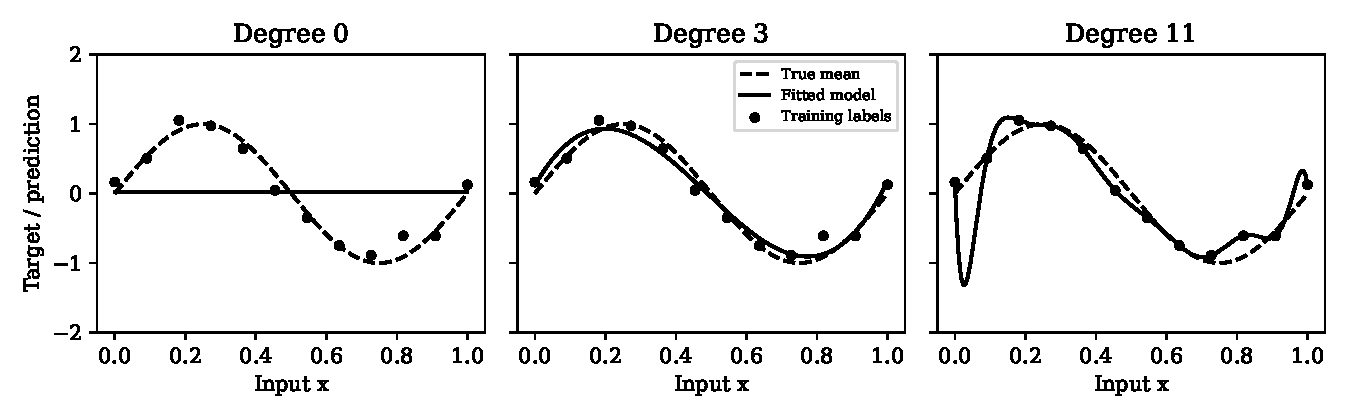
\includegraphics[width=.98\linewidth]{bias_variance/fits.pdf}
\caption{Constructed sine experiment: the same 12 noisy observations, with degrees 0, 3, and 11. Solid curves are fitted predictions; dashed curves are the conditional mean; dots are training labels. All panels share the plotted vertical range; extreme interpolating excursions may extend beyond it. Low training error alone does not certify accuracy between samples.}
\end{figure}

\subsection{Diagnosing generalization from results}
For $n_{\rm test}$ independent held-out examples, report
\[
\widehat R_{\rm test}=\frac1{n_{\rm test}}\sum_i(\hat f(x_i;\mathcal D)-y_i)^2,
\qquad \mathrm{RMSE}=\sqrt{\widehat R_{\rm test}}.
\]
MSE has squared target units; RMSE has target units. Compare like losses on comparable distributions. ``Low'' means low relative to a baseline, application tolerance, or attainable noise level, not a universal numeric threshold.
\begin{center}\small
\begin{tabular}{p{.24\linewidth}p{.32\linewidth}p{.33\linewidth}}
\toprule Pattern & Plausible diagnosis & Check before concluding\\\midrule
High training and test error & Underfitting / excessive restriction & Optimization failure, missing information, and high noise can also cause this.\\
Very low training error, much larger test error & Overfitting & Check leakage, sample size, and train--test distribution shift.\\
Low test error; modest gap & Useful generalization on this distribution & Check uncertainty, subgroup errors, and representative sampling.\\\bottomrule
\end{tabular}
\end{center}
The slide's ``perfect fit'' is a vivid example, not a necessary condition for overfitting. A model can overfit without zero training error. Similarly, underfitting is inadequate representation of the predictive structure, not merely failure to match every noisy label. A small train--test gap can coexist with very poor predictions. Plot residuals against $x$: systematic curvature suggests missing structure; large changes after resampling suggest instability. These are diagnostic clues, not isolated proofs.

\paragraph{Choosing $M$.} Fit coefficients on training data; compare candidate degrees on validation data or through cross-validation; evaluate the selected procedure once on an untouched test set. Repeatedly selecting degrees using test error turns that set into validation data. Even when only train and test results are supplied for diagnosis, this distinction matters for any subsequent model choice.

\paragraph{Predict before continuing (A2).} Three models have train/test MSE $(0.48,0.50)$, $(0.03,0.05)$, and $(0.0001,0.80)$ on comparable, sufficiently large splits. Which is the strongest candidate for each diagnosis? Can these numbers reveal the separate bias, variance, and noise components?
